%!TEX root = ../template.tex
%%%%%%%%%%%%%%%%%%%%%%%%%%%%%%%%%%%%%%%%%%%%%%%%%%%%%%%%%%%%%%%%%%%%
%% chapter4.tex
%% NOVA thesis document file
%%
%% Chapter with lots of dummy text
%%%%%%%%%%%%%%%%%%%%%%%%%%%%%%%%%%%%%%%%%%%%%%%%%%%%%%%%%%%%%%%%%%%%
\chapter{Implementation of the \textit{iCBD-Replication and Cache Server}}
\label{cha:impl_replication_caching}

This chapter addresses the implementation of the central topics of this thesis, divided into two major fields.
We first start with a section talking about the creation of a middleware system that provides replication features in an integrated way to the iCBD platform. While providing a detailed description of the concept and architectural model, as well as the implementation decisions, made along the accomplishment of this contribution.
Next, we show the work done on improving the performance of the platform clients. Displaying how setting up a client-side caching system that stores images adjacent to the consumers obtain that sought enhancements. Concluding in exploring the challenges of recreating the complete platform in a new environment and implementing a real-world scenario at Nova University Computer Science department laboratories.

%will at last state the problem and motivation for introduction replication techniques in the storage components of the platform. Moreover, the section prefaces the importance of the implementation of cache servers that hold part of the distribution burden and crucial for the support of an increased number of clients.

This chapter is partitioned as follows :

\begin{description}
    %
    \item [Section~\ref{sec:impl_replication}] overviews the implementation of the middleware dubbed iCBD-Replication. Beginning the journey through the initial architectural process and then showing the implemented components and their interaction with the several layers of the platform.
    %
    \item [Section~\ref{sec:impl_cache_server}] shows how the complete iCBD platform was installed in the NOVA University cluster. Then, a description of the work performed to include a client-side caching server directly connected to the final clients.
    %
\end{description}
\newpage


%%-------------------------------------------------------------------
%%	4 - Implementation of a Replication Module
%%-------------------------------------------------------------------
\section{Implementation of a Replication Module}
\label{sec:impl_replication}

One of the central objectives of iCBD is to provide a platform that can be both cloud-centric, with the administration and a portion of the storage burden gathered in a public cloud, or fully hosted on client premises. Either way, it becomes evident that data locality is an important subject, which means that there is the necessity to study how this data will flow between the multiple components of the iCBD platform.
As can be imagined, this is a data-intensive platform, boasting multiple storage devices in many networks and an array of consumers demanding that data at any given time.

All these factors allied to the platform architecture result in the need to create a new component, whose chief mission is to ensure that the data is correctly replicated in the appropriate places, maintaining the consistency of the various versions of the iCBD Machine Images stored.

%%-------------------------------------------------------------------
%%	4. - Requirements of the Module
%%-------------------------------------------------------------------
\subsection{Requirements of the Module}
\label{sub:requirements_icbdrep}

Since the beginning of this work, the file system selected for use in the storage layer was selected, this is due to the fact that, there was already a functioning prototype of the core iCBD platform making use of BTRFS for all data storage matters. The most critical feature for the operation of the platform is that the file system supports snapshots. BTRFS is a modern file system based on the copy-on-write (COW) principle \textbf{(CITATION NEEDED)} capable of creating lightweight copies of a file. We detailed the importance of this trait in Section~\ref{sub:icbd_architecture_storage}.
 
The condition described above applies only in the choice of the File System, in theory, any File System that supports snapshots can be employed in the platform. That is, in fact, the case with the work developed in a dissertation carried out in parallel to this one, where the focus is the use of an object-oriented file system, in particular, the CEPH File System.
Due to this imposition, it is key that this work makes the best use of the BTRFS features, exploring the incremental backup capabilities. More, the replication process should fully integrate with the core platform that already distributes iMIs to clients. Preservation of consistency of the iMIs is also a concern, assuring the distribution of new versions when they are created.

Moreover, it should be taken in account the locality of the data, since the communications could originate and end in the same data centre and the same local network, or happening between different locations that can be in opposite sides of the world. Such aspects as the bandwidth used and the encryption of the data becomes essential to address, requiring the examination of several compression algorithms that can be accommodated to the way the data is processed and also ways of keeping this data secure by encrypting the communications.
\newpage

%Requirements
%The file system is set BTRFS will be used.
%Many reasons for that:
%The most important is the support for snapshots
%Compression


%\subsubsection{Preliminary tests on the BTRFS Incremental Backup features}
\paragraph{Experimentation with the BTRFS Incremental Backup features}
\label{par:incremental_btrfs}

A first step is trying to understand the most efficient way to transfer this unique kind of data (i.e. an iMI). Given the fact that we are working with a file system with snapshots capabilities, we want to take advantage of this functionality and minimise the amount of data roaming the network.

The BTRFS developers provide a userspace set of utilities that can manage BTRFS filesystems, called \texttt{btrfs-progs}. Within that set of tools, there is a pair of commands, \texttt{btrfs send}~\cite{btrfs_send}, and \texttt{btrfs receive}~\cite{btrfs_receive}, that provides the capability to transport data via a stream and employ those differences in a remote filesystem. 

The send command facilitates the process of generating a stream of instructions that describe changes between two subvolume snapshots. Also available in the command is the ability to use an incremental mode, where given a parent snapshot that is available in both send and receive sides, only the small delta between snapshots (e.x. \textit{V2} and \textit{V2-1} in fig~\ref{fig:imi_snap}) is going to integrate the stream. This feature is outstanding since considerably reduces the amount of information that needs to be transferred to reconstruct the snapshot in the receiving end. The send side operations occur in-kernel, beginning by determining differences within subvolumes and based on those differences the kernel generates a set of instructions in a custom formulated stream.

\begin{figure}[htbp]
    \centering
    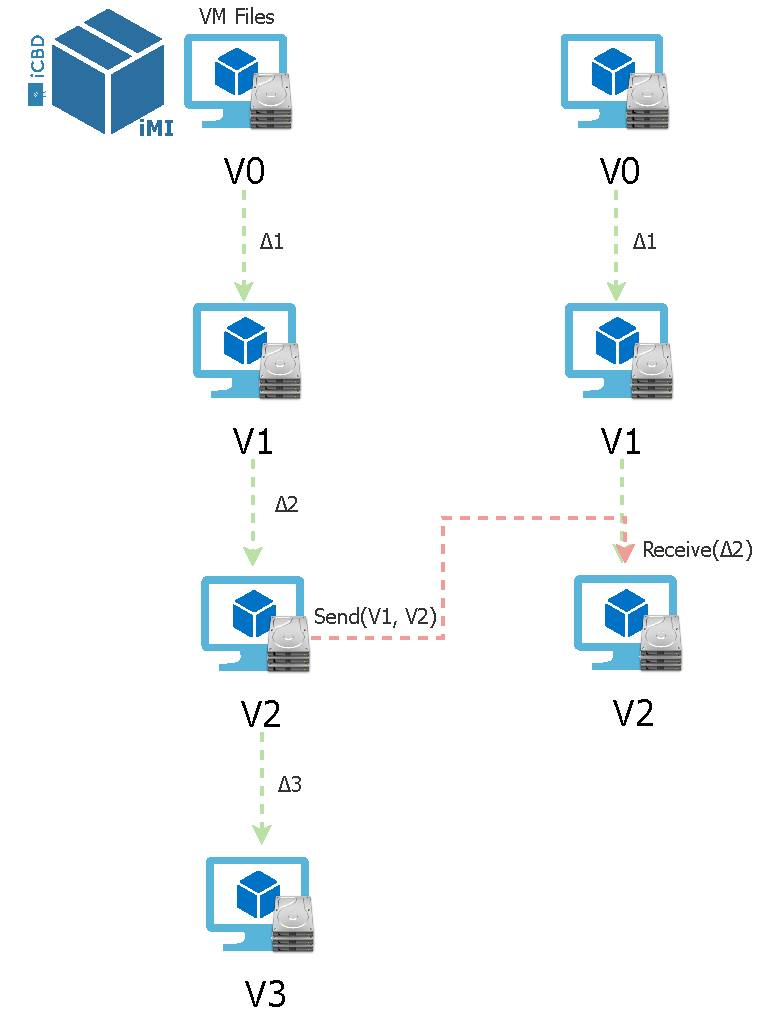
\includegraphics[height=4in]{cap4_iMI_deltas}
    \caption{iCBD iMI Snapshots Structure}
    \label{fig:imi_snap}
\end{figure}
\newpage

On the remote end, the received command accepts the stream generated by the send command and uses that data to recreate one or more snapshots. Contrary to the send command, receive executes in user space, replaying the instructions that come in the stream one by one, these instructions include the most relevant calls found in a Virtual File System, with Unix system calls like \texttt{create()}, \texttt{mkdir()}, \texttt{link()}, \texttt{symlink()}, \texttt{rename()}, \texttt{unlink()}, \texttt{write()}, along with others.~\cite{btrfs_design}


%https://btrfs.wiki.kernel.org/index.php/Incremental_Backup
%https://www.samba.org/ftp/rsync/rsync.html

%The first step is to try to understand the most efficient way to transfer this peculiar kind of data. Given the fact that we are working with a file system with snapshots capabilities, we want to take advantage of this functionality and minimise the amount of data roaming the network. In this sense, we next present some preliminary tests in multiple ways of transferring snapshots between BTRFS file systems both in the same machine and in different ones.
%The results obtained here conjugated with the defined requirements are essential for defining the architecture of the replication module steering the implementation at its best path.

%Before the start of any implementation, there was the need to validate the capabilities of the BTRFS file system regarding sending snapshots across different systems.
%As one of the requirements was the efficiency of the transference of data. So a small comparison was in order. 

%%-------------------------------------------------------------------
%%	4. - System Overview
%%-------------------------------------------------------------------
\subsection{System Overview}
\label{sub:system_overview}


\begin{figure}[htbp]
	\centering
	
\includegraphics[height=4in]{placeholder}
	\caption{iCBD Replication Architecture}
	\label{fig:icbd_rep_architecture}
\end{figure}

Since the replication module needs to interact with several bash scripts, with the core iCBD platform, including command line tools and some operating systems low-level features, we betted that the most suitable approach was creating a python distributed middleware using a master-replica paradigm.

Python as a programming language enjoys some valid idiosyncrasies, functioning as an object-oriented language, possessing an extensive standard library and enjoys a big community delivering packages with a wide range of functionality, all facts that contribute to make it the best programming language to bundle everything together.

The several modules of the middleware comprise the main functionalities allowing a node to behave as a Master or Replica node, where each one maintains its individual Image Repository. Then there are also a number of libraries that were developed to interface with some tools, as the BTRFS tool talked about above~\ref{par:incremental_btrfs}, to interface with an ssh connection, build wrappers for compression algorithms and even provide a REST API.

%%-------------------------------------------------------------------
%%	4. - Image Repository
%%-------------------------------------------------------------------
\subsection{Image Repository}
\label{sub:rep_image_repo}

This module presents itself with a central role in the replication process.

%\subsubsection{iCBD Snapshot Structure}
\paragraph{iCBD Snapshot Structure}
\label{par:icbd_snapshot}

In the replication module we treat a snapshot not only as raw data, but a collection of data and metadata that is essencial to unequivocally distinguish the multiple images present in the system. 


%%-------------------------------------------------------------------
%%	4. - Communications between nodes
%%-------------------------------------------------------------------
\subsection{Communications between nodes}
\label{sub:rep_comms}

The remote procedure call (RPC) supports inter-process communication and allows a procedure on a system to invoke a procedure running in a different address space, possibly on a remote system. RPCs were introduced in the early 1970s by Bruce Nelson and used for the first time at Xerox.


%\subsubsection{Pyro4 Library}
\paragraph{Pyro4 Library}
\label{par:rep_pyro4}

%https://pythonhosted.org/Pyro4/


\paragraph{TCP Sockets}
\label{par:rep_tcp_sockets}

\paragraph{Secure Shell Protocol (SSH)}
\label{par:rep_ssh}


%%-------------------------------------------------------------------
%%	4. - Stream Compression
%%-------------------------------------------------------------------
\subsection{Stream Compression}
\label{sub:rep_stream_compression}

\paragraph{Snappy}
\label{par:rep_snappy}

\paragraph{LZ4}
\label{par:rep_lz4}


%%-------------------------------------------------------------------
%%	4. - Master Node
%%-------------------------------------------------------------------
\subsection{Master Node}
\label{sub:rep_master_node}

\paragraph{Keep Alive}
\label{par:rep_keep_alive}

\subsubsection{CLI Interface}
\label{subsub:rep_cli_interface}

\subsubsection{REST API}
\label{subsub:rep_restapi}

%%-------------------------------------------------------------------
%%	4. - Replica Node
%%-------------------------------------------------------------------
\subsection{Replica Node}
\label{sub:rep_replica_node}






%%-------------------------------------------------------------------
%%	4. - Building a iCBD Cache Server
%%-------------------------------------------------------------------
\section{Building a iCBD Cache Server}
\label{sec:impl_cache_server}

%To solve some of the enunciated problems with a DaaS solution that derive from limited bandwidth, latency and jitter from the limitation of accessing the image repositories from an internet connection and provide some scalability feature with the implementation of proximity cache servers are key. These cache servers can store replicas of the iMIs created and maintained in an administration server. Moreover, since they are located in the same LAN segment as the clients is from here that they will boot.
%For accomplishing this work, the cache servers need to have hard drives. (Although it would be possible to have diskless cache servers, they would be blocked if there was an interruption in the internet access, and it is to avoid that the local drives are necessary. )

%A instalação, configuração e administração dos cache-servers far-se-á também pela instanciação a partir da imagem de uma VM especialmente preparada para o efeito e residente na cloud, no sistema de administração. Os cache-servers arrancam inicialmente pela rede a partir do servidor na cloud e carregam um Linux que vai formatar os discos, neles instalando o conteúdo da própria imagem de VM, terminando com a instalação de um boot loader que irá arrancar o sistema do cache-server após a máquina fazer reboot. Daí em diante o sistema de administração na cloud irá disponibilizar as actualizações que forem necessárias, podendo mesmo forçar a re-instalação total dos cache-servers.

%Note-se que uma vez instalado um cache-server numa LAN, dada a grande fiabilidade que pode ser ainda reforçada através das técnicas habituais em sistemas tolerantes a faltas e de elevada disponibilidade (referir a sugerida pelo Paulo), torna-se viável a utilização de servidores diskless, instanciados a partir de VMs templates configuradas e administradas na cloud e depois replicadas para o cache-server, como nas imagens dos desktops.

%Assim como o Linux dos cache-servers é instalado nos discos locais dos servidores a partir de imagens na cloud, é possível fazer o mesmo com qualquer outra imagem de Linux que se queira. Assim, o administrador de sistema de um cliente poderá configurar outras VMs com o software e os serviços de que necessitar, designar uma máquina física como alvo, e fazer com que a VM seja vertida para os discos da sua máquina física, sendo configurado um boot loader para lhe permitir arrancar com essa configuração.

%Como os clientes nestas categorias tipicamente necessitam de dezenas, centenas ou mais de postos de trabalho, na prática é impossível suportá-los directamente a partir de repositórios remotos de VMs templates. Em vez disso, iremos recorrer a “servidores de proximidade” ou “c​ache-servers”​, máquinas Linux reais ou virtuais devidamente dimensionadas e configuradas, instaladas na LAN dos clientes, idealmente uma (ou mais) por cada segmento de rede, as quais manterão réplicas das VMs templates a que cada cliente tem acesso nos repositórios remotos.
%Com estes cache-servers localmente acessíveis aumentar-se-á drasticamente a velocidade de transferência de dados e a latência e o jitter nos acessos reduzir-se-ão a valores insignificantes, podendo cada cache-server suportar dezenas (ou mais) de PCs clientes (estimamos o número em 15 a 30 por cada interface gigabit nos cache-servers, estimativa que permanece válido para PCs clientes ligados a 100 Mbps através de switches com ligação gigabit aos cache-servers).


\subsection{The infrastructure}
\label{sub:infrastructure}

%Machines List:
%TODO
%Servers - 2x HP ProLiant DL380 Gen9
%Switch - HPE flexfabric 5700 jg898a
%Disk array - HPE MSA 2040 SAN Storage

\begin{table}[htpb]
\centering
\begin{tabular}{lcc}
\hline
                               & \textbf{FCT NOVA}          & \textbf{Reditus}           \\ \hline
\textit{\textbf{Servers}}      & 2 x HP ProLiant DL380 Gen9 & 2 x HP ProLiant DL380 Gen9 \\
\textit{\textbf{Switch}}       & HPE flexfabric 5700 jg898a & HPE flexfabric 5700 jg898a \\
\textit{\textbf{Disk Array}}   & HPE MSA 2040 SAN Storage   & -                          \\
\textit{\textbf{WorkStations}} & 2 Labs (15 PCs each)       & 3 Test PCs                 \\
\textit{\textbf{Networking}}   & 1 Gbps                     & 1 Gbps                     \\ \hline
\end{tabular}
\caption{Physical infrastructure in both sites}
\end{table}


\subsection{System Overview}
\label{sub:system_overview}

%%-------------------------------------------------------------------
%%	4. - Services
%%-------------------------------------------------------------------
\subsection{Services}
\label{sub:cache_services}


%%-------------------------------------------------------------------
%%	4. - Networking
%%-------------------------------------------------------------------
\subsection{Networking}
\label{sub:cache_networking}

%%-------------------------------------------------------------------
%%	4. - Extra Efforts
%%-------------------------------------------------------------------
\subsection{Extra Efforts}
\label{sub:extra_efforts}

Found a Centos 7 kernel bug.
%https://bugs.centos.org/view.php?id=14228
%https://bugzilla.redhat.com/show_bug.cgi


GitLab

Since the work mainly goes around replication and infrastructure problems, makes all sense to think in how the base code is handled. Thinking on this subject and evaluating the code backup system in place (talk about what is the system in place), an svc system is ideal to what we what to accomplish.
So a GitLab on-premises system was deployed and configured. Also configured multiple repositories that will back each module of the iCBD platform.
There are two main objectives of this premise.
First, provide a safe environment for backing up all the base code of the modules. As well as provide versioning control of the that same code.
Second, facilitate a way to replicate the base code of the multiple modules though the various infrastructures running the icbd platform in a clean and transparent way.
Talk a bit of git vantages. (Replication possibilities, backing with the cloud..)
How is implemented? (VM in reditus infra..)



